\subsection{Implementaciones en código}

\subsubsection{Resolución de sistemas}

Para resolver los sistemas, armamos el método \textbf{resolver$\_$sistema}, el cual toma una matriz $m$, un booleano \newline
$triangular\_i$ indicando si es triangular superior o inferior, y un vector $b$. El objetivo es que retorne el vector solución.

\subsubsection{Resolución Gauss}
\textbf{resolver\_gauss} recibe la matriz $m$ a triangular y el vector $b$. Ejecuta el método de Gauss y después se le pasa la matriz triangulada extendida resultante a \textbf{resolver\_sistema} para recibir finalmente el vector solución. 

\subsubsection{Resolución LU}
A diferencia de \textbf{resolver\_gauss}, podemos aprovechar que solo hace falta una única corrida del método LU a un sistema para poder resolver cualquier otro. Por ende, para situaciones donde haya muchas instancias a resolver, realizamos una única vez LU para la primera instancia (por fuera del \textbf{resolver\_lu}, está en la función \textbf{main}). Luego utilizamos las matrices resultantes L y U como parámetros para \textbf{resolver\_LU}. 

\subsubsection{Isoterma y peligrosidad}

Pensamos en algo sencillo para \textbf{buscar la isoterma}: que busque el valor más cercano en todos los radios. Dicho de otra manera, dada una isoterma $iso$, $r_i$ radios con i = 0,..,$m$ y $temp(r_{i}, \theta)$ la temperatura en el punto $(r_i, \theta)$, vamos a proponer que la isoterma en $r_i$ sea aquel número que tenga la menor diferencia con el valor buscado:

\begin{equation}\label{ecuacion_isoterma}
     isoterma(r_{i})  = min(|iso - temperatura(r_{i}, \theta)|)
\end{equation}

Para la \textbf{peligrosidad}, en una primera instancia pensamos que el sistema se considerará peligroso si algún punto de la isoterma se encuentra dentro del tercio de radios más cercanos a la pared exterior. 

\

Analizando posibles fallas, notamos lo siguiente: si pensamos en un sistema donde uno de los sensores falla y detecta la isoterma cerca a la pared exterior, este sistema sería equivalente a uno en donde toda la isoterma esté cerca de la pared exterior. Por ello, reconsideramos algo más realista, que verifique si un sector de la isoterma está en el tercio más cercano; es decir, si un ángulo de la isoterma se encuentra en el tercio más cercano, y \emph{también} sus ángulos aledaños lo están. En este caso, se puede considerar el que no se trata de un fallo de un sensor, sino una posible situación de riesgo.

\subsection{Experimentos}

A continuación vamos a detallar los experimentos realizados y los datasets creados para cada uno. Los experimentos fueron corridos en una computadora con las siguientes especificaciones: 

\begin{itemize}
    \item Ubuntu 20.04.4 LTS 64-bit, 14,0 GiB Memory, Intel Core i5-3570,
    \item Ubuntu 20.04.4 LTS 64-bit, 15,6 GiB Memory, AMD Ryzen 3 2200g.
\end{itemize}

Tomamos las siguientes decisiones a la hora de crear los datasets para los experimentos:
\begin{enumerate}
    \item Para los valores de los radios $r_i$ y $r_e$ decidimos tomar los mismos valores constantes a lo largo de los experimentos debido a que es posible armar sistemas equivalentes para distintos valores de los radios, 
    \item El valor de la isoterma será de 500, tal como se menciona en el enunciado,
    \item Los valores que iremos modificando serán la cantidad de radios y cantidad de ángulos, los valores de las temperaturas de las paredes internas y externas, y la cantidad de instancias.    
\end{enumerate}

\newpage

\subsubsection{Experimento 1: Prueba de modelo}

La idea del \emph{primer experimento} consiste en encontrar los valores de $m$ y $n$ para obtener la "mejor" discretización: que muestre un gráfico lo suficientemente fino y que conseguirlo no sea muy costoso temporalmente.  

\

Para este experimento solo vamos a utilizar Gauss dado que al tener una sola instancia por archivo, no podemos aprovechar las ventajas del método LU. Una sola instancia de LU sería lo mismo que resolver el sistema con Gauss (con el adicional de algunas operaciones extra). 

\

Nuestro objetivo será encontrar una discretización tal que la posición calculada de la isoterma sea lo más cercana posible a la real, sin excedernos computando instancias cuyo rendimiento sea decreciente considerando el tiempo de computo de la misma y la precisión que se obtenga. Por ello, para este dataset dejaremos fijo el valor de $n$ (ángulos) y modificaremos los valores de $m$, incrementando la cantidad de radios. Nuestra \textbf{hipótesis} será que con $n$ = 40, podremos encontrar un valor de $m$ tal que  la discretización es lo suficientemente fina como para estar cerca de la isoterma real, y que a su vez calcularla no tarda demasiado. 

\

Para decidir qué $m$ elegiremos, calcularemos las posiciones de las isotermas de los hornos resultantes, iremos comparando los resultados con la instancia anterior y analizaremos a partir de qué momento la diferencia se hace despreciable.  


\begin{itemize}
    \item[-] Este primer dataset contempla una discretización del horno con temperaturas fijas $T_i = 1500~$ y $~T_e = 200$,
    \item[-] $n = 40$,
    \item[-] $m \in \{x~:~x = i\cdot 2, ~ i = 2\ldots20\}$,
    \item[-] $ninst = 1$, con tantos archivos como las instancias que surgen de los pares $(m,n)$,
    \item[-] $isoterma = 500$, 
    \item[-] $r_i = 10$,
    \item[-] $r_e = 15$.
\end{itemize}

\subsubsection{Experimento 2: Prueba de cómputo}

Una vez conseguida la discretización buscada, nos propusimos armar un \emph{segundo experimento} con el objetivo de decidir cuál método de resolución es el óptimo entre Gauss y LU. Para ello, armamos un dataset en donde el horno va cambiando con el tiempo, es decir, el archivo en cuestión tiene 30 instancias del mismo horno. 

\

Adicionalmente, las temperaturas de las paredes respetan una distribución normal para simular un posible error de medición en los sensores con $\sigma = \frac{\mu}{50}$. 

\

Con esto, creamos el \textbf{Dataset 2: Temperaturas que cambian con el tiempo}, con las siguientes características:

\begin{itemize}
    \item[-] $n = 40$,
    \item[-] $m = 30$,
    \item[-] $ninst = 30$,
    \item[-] $isoterma = 500$,
    \item[-] $r_i = 15$,
    \item[-] $r_e = 5$,
    \item[-] $T_i \sim N(1500, 30)$,
    \item[-] $T_e \sim N(200, 4)$,
\end{itemize}

\

Para este dataset aplicaremos Gauss y LU, con la \textbf{hipótesis} de que LU va a tardar mucho menos que Gauss.

\subsubsection{Experimento 3A: Prueba de riesgo}

Investigando sobre el funcionamiento de altos hornos, encontramos que los materiales que constituyen sus paredes son resistentes al calor. Teniendo esto en cuenta, pensamos en distintos motivos por los cuales podría haber un accidente, y pensamos un \emph{tercer experimento} en donde tenemos un alto horno con paredes construidas de materiales de baja calidad, los cuales tienen un límite de resistencia y utilizan un sistema de refrigeración pero el mismo \emph{falla}, y mitad del horno comienza a incrementar su temperatura con el pasar del tiempo.

\

Nuestro objetivo es ver cómo cambia la isoterma cuando hay una diferencia de temperaturas irregular en una zona considerable del horno a través del tiempo y observar cómo afecta este cambio en el sistema.

\

Vamos a utilizar la discretización hallada en el primer experimento, con el método LU, dado que vamos a usar el mismo sistema con los mismos coeficientes aprovechando lo hallado en los dos experimentos anteriores.

\

Utilizar LU será más eficiente, dado que solamente la primera instancia se ejecuta con tiempo O($n^3$), y todas las posteriores se ejecutaran en O($n^2$).

\

Nuestra \textbf{hipótesis} es que creemos que la isoterma va a perder su forma circular, y empieza a deformarse hacia la zona de temperaturas más altas, acercándose al borde con temperaturas más altas con el paso del tiempo de la siguiente forma:

\

\begin{figure}[h]
    \begin{center}
    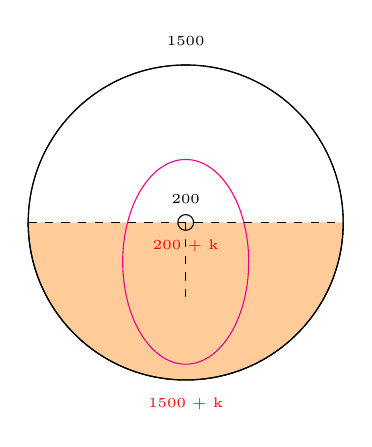
\begin{tikzpicture}
        \draw (0,0) circle [radius=2];
        \filldraw[fill=orange!40!white] (-2,0) arc (-180:0:2);
        \draw[magenta] (0,-0.5) ellipse [x radius=0.8, y radius = 1.3];
        \draw (0,0) circle [radius=0.1];
        \draw (0,0) circle [radius=2];
        \draw[dashed] (-2,0) -- (2,0);
        \draw[dashed] (0,0) -> (0,-1);
        \node at (0,2.3) {\tiny 1500};
        \node at (0,0.3) {\tiny 200};
        \node[red] at (0,-0.3) {\tiny 200 + k};
        \node[red] at (0,-2.3) {\tiny 1500 + k};
    \end{tikzpicture}
    \caption{Esbozo gráfico de la hipótesis}
    \label{fig:hipotesis}
    \end{center}
\end{figure}

donde $k$ es el incremento de temperatura que se percibe. Para corroborar esto creamos el \textbf{Dataset 3: Horno con sistema de refrigeración no funcional} de las siguientes características:

\begin{itemize}
    \item[-] $n = 40$,
    \item[-] $m = 30$,
    \item[-] $ninst = 50$,
    \item[-] $isoterma = 500$,
    \item[-] $r_i = 10$,
    \item[-] $r_e = 15$,
    \item[-] $T_i = 1500$,
    \item[-] $T_e = 200$,
    \item[-] $k = 10$, este $k$ es el incremento de temperatura que sufre la mitad del horno en cada instancia.
\end{itemize}


\subsubsection{Experimento 3B: Prueba de sensado}

En este experimento queremos atestiguar cómo influye en el sensado de la isoterma el que haya sensores defectuosos en el horno. Para lograr esta situación, contemplamos que en sensores tomados al azar, el desvío que manejen sea mucho mayor que el de los sensores en correcto funcionamiento.

\

Creamos el \textbf{Dataset 4: Horno con sensores fallados} con las siguientes características, donde $SF$ es la temperatura que manejan los sensores fallados:

\begin{itemize}
    \item[-] $n = 40$,
    \item[-] $m = 30$,
    \item[-] $ninst = 30$,
    \item[-] $isoterma = 1000$,
    \item[-] $r_i = 15$,
    \item[-] $r_e = 5$,
    \item[-] $T_i \sim N(1500, 30)$,
    \item[-] $T_e \sim N(500, 4)$,
    \item[-] $SF \sim N(500, 100)$,
\end{itemize}

\

Aclararemos que para cada generación del dataset, dichos sensores defectuosos son elegidos al azar, y no cambian a lo largo de las instancias. 

\

Para este dataset aplicaremos LU, con la \textbf{hipótesis} de que se podrán distinguir perturbaciones en la forma de la isoterma en los sensores defectuosos.
